\documentclass{article}
\usepackage{graphicx}
\usepackage{color}
\usepackage{psfig}
\usepackage{times}
\usepackage{setspace}
\usepackage{url}
%\usepackage[final]{pdfpages}
%\usepackage{verbatim}
%\usepackage{chapterbib}
%\usepackage{ifthen}
%\usepackage{longtable,lscape}
\begin{document}
\title{The Title}
\author{
Allen Day \and Jun Dong \and Stanley F. Nelson
% Allen Day\correspondingauthor$^{1,2,\ddag}$ \email{Allen Day\correspondingauthor - allenday@ucla.edu} \and
% Brian D. O'Connor$^{2,3,\ddag}$ \email{Brian D. O'Connor - boconnor@ucla.edu} \and
% Jordan Mendler$^{1}$ \email{Jordan Mendler - jmendler@ucla.edu} \and
% Jared Fox$^{1,4}$ \email{Jared Fox - jaredfox@ucla.edu} \and
% Stanley F. Nelson$^{1}$ \email{Stanley F. Nelson - snelson@ucla.edu} \and
% Lincoln D. Stein\correspondingauthor$^{2}$  \email{Lincoln D. Stein\correspondingauthor - lstein@cshl.edu}
}
\maketitle

\section{Abstract}\label{Abstract}
...

\section{Introduction}
\label{Hypothesis}
%Genes can be annotated by observing their expression pattern across a large
%number of anonymous, unlabeled samples.  Further, we assert that
%non-orthologous genes can be annotated cross-species given 1) gene expression
%observations in two species, and 2) a partial, sequence-based ortholog map
%between the two species.

\section{Methods}\label{Methods}

% <execute lang="bash">
% wc -l /home/allenday/cvsroot/celsius/dump/data2/HG-U133_Plus_2.rma.sxe.col | awk '{print $1}' > m0_col.tex
% wc -l /home/allenday/cvsroot/celsius/dump/data2/HG-U133_Plus_2.rma.sxe.idx | awk '{print $1}' > m0_row.tex
% </execute>

\subsection{Data Processing}\label{Processing}
We retrieved RMA-processed gene expression data for the HG-U133\_Plus\_2
arraydesign from the Celsius microarray data warehouse
(\url{http://genome.ucla.edu/projects/celsius}) \cite{rma,celsius}.  In total,
there were 12826
 arrays $S$, each of which reports measurements for 54675

probesets $P$.  We denote this initial $S{\times}P$ matrix as $M$.

It was clear from a cursory examination of summary statistics prepared from $M$
that there were abberant arrays present, and that these arrays would have a
negative impact on any downstream analyses.  At a coarse level, there appeared
to be XXX types of aberrant arrays:

\renewcommand{\labelenumi}{\Alph{enumi}.}
\begin{enumerate}
\item arrays with extremely high gene expression values across many probesets.
\item arrays with extremely low gene expression values across many probesets.
\item arrays with dissimilar expression values for two probesets reputedly
measuring the same gene.
%\item arrays with dissimilar expression values for genes known to be
%co-expressed (Section \ref{corpass}).
\end{enumerate}

We sought to remove these abberant arrays from the dataset.

% <execute lang="R">
% z             = read.table('/home/allenday/cvsroot/celsius/dump/data2/HG-U133_Plus_2.rma.sxe.summary2')
% trim.fraction = 10;
% brightdim.cutoff = 3;
% trim.length   = as.integer(length(z[,5]) / trim.fraction)
% z5            = sort(z[,5]);
% z5.trim       = z5[ trim.length:(length(z5)-trim.length) ]
% postscript('array_means.ps',width=8,height=8,horizontal=FALSE,onefile=FALSE,paper="special",encoding="TeXtext.enc")
% hist(z5.trim,breaks=50,xlab="mean probeset intensity",ylab="frequency",main="mean probeset intensity of arrays")
% dev.off()
% write(trim.fraction, 'trim_fraction.tex');
% write(brightdim.cutoff, 'brightdim_cutoff.tex');
% write(mean(z5.trim),'trimmed_means_mean.tex');
% write(sd(z5.trim),'trimmed_means_sd.tex');
% write(sum( (z5 - mean(z5.trim)) / sd(z5.trim) >  brightdim.cutoff ),'bright_count.tex')
% write(sum( (z5 - mean(z5.trim)) / sd(z5.trim) < -brightdim.cutoff ),'dim_count.tex')
% write(sum( (z5 - mean(z5.trim)) / sd(z5.trim) < -brightdim.cutoff ) + sum( (z5 - mean(z5.trim)) / sd(z5.trim) >  brightdim.cutoff ),'brightdim_count.tex')
% write((1:length(z[,5]))[(z[,5] - mean(z5.trim)) / sd(z5.trim) > 3 | (z[,5] - mean(z5.trim)) / sd(z5.trim) < -3],'/home/allenday/cvsroot/celsius/dump/data2/HG-U133_Plus_2.rma.sxe.brightdim',ncolumns=1);
% </execute>
%% <execute lang="bash">
%% /home/allenday/cvsroot/celsius/dump/bin/i386-redhat-linux-gnu.4/trim.exe 54675 /home/allenday/cvsroot/celsius/dump/data2/HG-U133_Plus_2.rma.sxe.brightdim /home/allenday/cvsroot/celsius/dump/data2/HG-U133_Plus_2.rma.sxe.dat data2/HG-U133_Plus_2.rma_trim1.sxe.dat 
%% /home/allenday/cvsroot/celsius/dump/bin/trim_index.pl /home/allenday/cvsroot/celsius/dump/data2/HG-U133_Plus_2.rma.sxe.brightdim /home/allenday/cvsroot/celsius/dump/data2/HG-U133_Plus_2.rma.sxe.idx /home/allenday/cvsroot/celsius/dump/data2/HG-U133_Plus_2.rma_trim1.sxe.idx 
%% cp /home/allenday/cvsroot/celsius/dump/data2/HG-U133_Plus_2.rma.sxe.col /home/allenday/cvsroot/celsius/dump/data2/HG-U133_Plus_2.rma_trim1.sxe.col 
%% </execute>
% <execute lang="bash">
% wc -l /home/allenday/cvsroot/celsius/dump/data2/HG-U133_Plus_2.rma_trim1.sxe.col | awk '{print $1}' > m1_col.tex
% wc -l /home/allenday/cvsroot/celsius/dump/data2/HG-U133_Plus_2.rma_trim1.sxe.idx | awk '{print $1}' > m1_row.tex
% </execute>

\subsubsection{Removal of Dim and Bright Arrays}\label{dimbright}

Class A \& B arrays were easiest to identify.  We calculated the mean
expression value of all probesets for each array, then calculated the mean and
standard deviation of a 10
\% trimmed distribution of those
means.

The trimmed means had a mean of 231.1081
 and a standard
deviation of 21.01693
.  A histogram of the distribution is
given in Figure \ref{figure:means}.

%%%% XXX this belongs in a higher-level or dedicated section.
%To get around this problem of co-processing, Katz \emph{et al.} described a
%method for large scale, iterative processesing of Affymetrix microarrays
%\cite{genelogic}.  Because multi-array methods for performing background correction

%ok
Microarray pre-processing, also known as \emph{quantification}, is the process
of estimating the quantity of each gene in the sample that was assayed in the
hybridization step (Section \ref{Hybridization}) of the experiment.
Quantification can be broken down into four distinct sub-procedures, executed
in the following order: image processing, background correction, normalization,
and summarization.  Much of the specific details in this section are
idiosyncratic to the Affymetrix GeneChip platform, but general principles apply
to all forms of microarray technology.

%ok
\subsection{Image Processing}\label{Image Processing}

The term \emph{image processing} is used to describe a set of steps that
transforms the physical microarray into a digital file suitable for subsequent
processing by a computer.  The techical details of the protocol vary, but the
general principles described here remain the same.

As discussed in Section \ref{Hybridization}, fluorescent dyes are linked to the
synthesized DNA sequences that are hybridized to the microarray.  The
microarray is placed in a digital scanning apparatus that contains laser(s)
that can emit light at the excitatory frequency of each dye.  The apparatus
also contains photosensors that are able to detect the fluorescent light from
the dye(s).  Each laser, then, is scanned across the surface of the microarray
and the photosensors record the position and intensity of light for each dye.
The raw form of these data is typically a series of images encoded using a
lossless format, such as TIFF.  The image is then processed by an alignment
algorithm that aligns the captured image to the coordinate system known to have
been printed/synthesized onto the microarray surface.

Finally, platform-specific protocols are used to represent the raw image in a
format more suitable for downstream processing.  For example, with
single-channel Affymetrix microarrays, the TIFF image is converted to an
alternate format, called \emph{CEL} format, that describes the attributes of
each microaray feature, such as mean intensity, variance, and number of pixels
that represent the feature.

%ok
\subsection{Background Correction}\label{Background Correction}

Background correction is a statistical procedure that estimates and removes low
levels of noise on the microarray.  Background noise can have many sources.

The simplest and most common source of background noise is optical.  It can be
caused by general cross-hybridization of target to all probes, mis-calibration
of the microarray scanner's photo-sensor, and diffused or reflected light from
the laser used to excite the fluorescent dyes.  Optical noise can be estimated
by measuring the level of fluorescence from featureless regions of the
microarray and negative control probes that are not reverse-complementary to
any sequences in the hybridization mixture.  These measure background-level
reflected light and the level of non-specific hybridization, respectively.

Manufacturing and hybridization artifacts, such as surface scratches and salt
residues, are another source of noise.  A simple form of location-based
background correction is descibed in the Statistical Algorithms Description
Document \cite{affy:tech:2002}.   Briefly, the chip is broken into a $4x4$
grid of 16 rectangular regions.  The lowest 2\% of each region's probe
intensities are used to compute a background value for that region.  Each probe
(PM and MM) is then adjusted based upon a weighted average of the backgrounds
for all regions. The weights are based on the distances between the location of
the probe and the centroids of all regions.  More sophisticated methods attempt
to detect areas of the microarray containing high levels of manufacturing and
hybridization noise.  Noisy areas can be identified because the probes located
there will be outliers relative to probes for the same target located elsewhere
on the microarray.  Probes in these areas are considered unreliable and are
either given a very low weight parameter or are removed from normalization
(Section \ref{Normalization}) and other downstream processing (Section
\ref{Summarization}) altogether \cite{affyplm}.

Newer, multi-array background correction methods have leveraged existing data
to build a models of how background noise is generally distributed.  The gcRMA
model \cite{gcrma} includes a parameter the sequence composition of each probe,
while other models such as those used in the RMA and MBEI (dChip)
\cite{rma,mbei,dchip,vsn,bioc} methods only include a parameter for concordant
each probe is with other probes in the same set.  The RMA background correction
method is the \i{de facto} standard, and corrects perfect match (PM) probe
intensities by using a global model for the distribution of probe intensities
\cite{rma,gautier}.

%The model is suggested by looking at plots of the empirical distribution of
%probe intensities.  In particular the observed PM probes are modeled as the sum
%of a normal noise component N (Normal with mean $\mu$ and variance $\sigma^2$)
%and a exponential signal component S (exponential with mean $\alpha$). To avoid
%any possibility of negatives, the normal is truncated at zero. Given we have O
%the observed intensity, this then leads to an adjustment, given in Equation
%\ref{rmabg}:
%
%\begin{equation}
%\label{rmabg}
%E\left(s \lvert O=o\right) = a + b \frac{\phi\left(\frac{a}{b}\right) - \phi\left(\frac{o-a}{b}\right)}{\Phi\left(\frac{a}{b}\right) + \Phi\left(\frac{o-a}{b}\right) - 1 }
%\end{equation}
%
%where $a =  s- \mu - \sigma^2\alpha$ and $b = \sigma$. Note that $\phi$ and
%$\Phi$ are the standard normal distribution density and distribution functions
%respectively.  Note also that MM probe intensities are not corrected by either
%of these routines \cite{rma,bioc}.

Multi-array background correction methods are able to detect background noise
due to the manufacturing and hybridization artifacts described above, but the
size of the aray artifact can be as small as a single feature.  This should in
principle do a better job of noise estimation.  A major drawback to multi-array
background noise models is that the noise estimates are only valid in the
context of the co-processed set of microarrays.  This is because the noise
estimates are derived from parameter estimates specific to that set of
microarrays.  While this is not a problem for small-scale analysis on
individual experiments, it creates difficulties when merging data from multiple
experiments because all microarrays will need to be re-processed to re-fit the
parameters of the noise model.  This re-processing problem can become
intractable for background correcting a very large number of arrays.  Further
attention is given to tractability in Section \ref{Scalability}.

%ok
\subsection{Normalization}\label{Normalization}

After correcting for background noise (Section \ref{Background Correction}),
microarrays are normalized.  The purpose of normalization is to transform the
distribution of microarray measurements so that properties of the distribution
of measurements match expectations (e.g., a log-normal distribution).

The most simple form of microarray normalization is a linear scaling.  The
Affymetrix MAS 5 algorithm \cite{mas5} performs linear scaling by (1) setting
aside the top and bottom 1\% of measurements as outliers, adjusts the mean of
the remaining measurements to a constant value, then multiplies each
measurement, including the outliers, by the factor used to adjust the mean.

The normalization method used in the dChip software \cite{mbei,dchip} selects a
baseline microarray.   Then, all microarrays are normalized by selecting
invariant sets of probes within each of the ``treatment'' and ``baseline''
conditions.  These are used to fit a non-linear relationship between the two
conditions, and this relationship is used to carry out the normalization.

Many other normalization methods exist.  The essentially differ in two aspects:
the theoretical model of how the microarray behaves, and the techniques used to
fit the observed data to that model.  In this regard, normalization techniques
are similar to those used for background correction (Section \ref{Background
Correction}) and summarization (Section \ref{Summarization}).

A comparison of the performance of a larg number of normalization methods at
correctly estimating RNA concentration on a standard, synthetic data sets
published by Affymetrix is described in \cite{affybench}.

\subsection{Summarization}
\label{Summarization}

The last step in microarray data preprocessing is to combine the measurements
from all probes in a probe set into a single value.  This procedure is called
\emph{summarization}.

The simplest summarization algorithm, called ``average difference''
\cite{affy4} computes the mean of difference between each PM/MM probe pair
(Equation \ref{avgdiffsummary}),

\begin{equation}
\label{avgdiffsummary}
y_{k} = I_i^{-1}{\sum_{i=1}^{I_k} |PM_i-MM_i|}
\end{equation}

where the probe set $k$ has $PM$ perfect match and $MM$ mismatch probe pairs $i
= 1,\dots,I_k$.

Summarization methods parallel background correction and normalization methods
in that there are two varieties, the single-array methods and the multi-array
methods.  ``Average difference'' is an example of the former.  Multi-array
methods consider the distribution of probe measurements across all arrays, and
in some cases assign an array-specific parameter used to compute the probe set
summary.  The summarization component of the MBEI method introduced by Li and
Wong \cite{mbei,dchip} is given in Equation \ref{mbeisummary},

\begin{equation}
\label{mbeisummary}
y_{ij} = \phi_i \theta_j + \epsilon_{ij}
\end{equation}

where $y_{ij}$ is $PM_{ij}$ or the difference between $PM_{ij}-MM_{ij}$. The
$\phi_i$ parameter is a probe response parameter and $\theta_j$ is the
expression on microarray $j$.

The summarization component of RMA pre-processing \cite{rma} performss a
multi-array linear fit to data from each probe set.  Specifically, for probe
set $k$ with $i=1,\dots,I_k$ probe pairs and microarrays $j=1,\dots,J$ the
model given in Equation \ref{medianpolish} is fit,

\begin{equation}
\label{medianpolish}
\log_2\left(PM^{(k)}_{ij}\right) = \alpha_i^{(k)} + \beta_j^{(k)} + \epsilon_{ij}^{(k)}
\end{equation}

where $\alpha_i$ is a probe effect and $\beta_j$ is the $\log_2$ expression
value, and the method is known as \emph{median polish}, named after Tukey's
algorithm used to perform the calculation.

It is noteworthy that summarized probe set values from all popular multi-array
summarization methods, including those described here, are dependent upon the
probe set and microarray effect parameters calculated as part of the model fit.
While this is not a problem theoritically, it introduces unique challenges in
the implementation of a pre-processing pipeline for a large number of arrays.
This is discussed in greater detail in Section \ref{Scalability}.

\subsection{Scalability}\label{Scalability}

While the superiority of multi-array techniques described in Sections
\ref{Background Correction}-\ref{Summarization} has been established, a major
impediment to implementing these in practice is that they are not designed to
scale to large data sets due to the amount of system resources consumed by a
single quantification process.  One approach to solving this problem is
``divide and conquer''.  By breaking the matrices up row- or column-wise,
larger batches of microarrays can be co-processed \cite{aroma}.  While this is
useful for performing analysis on a static data set, it does not address the
needs of users performing analysis on constantly growing data sets, because
each time an additional microarray is added the entire set must be reprocessed.
Katz \emph{et al.} \cite{genelogic} recognized that the true advantage of
multi-array over single-array quantification methods is that they fit probe and
probeset behavior to a model, and that if a theoretical (as opposed to
emperical) model is used and reasonable estimates can be calculated and saved,
arrays can be added one by one without reprocessing the whole set.  A similar
system was implemented in Celsius, and is described in greater detail in
Chatper \celsiuschapter \cite{celsius}.


There were 726
 arrays with mean a expression value more
than 3
 standard deviations away from the mean of
trimmed means.  These were primarily dim arrays (n=711
) but there
were also bright arrays (n=15
).  These arrays were removed
from further consideration, leaving a matrix $M\prime$ with 12100

arrays and 54675
 probesets.

\subsubsection{Removal of Inconsistent Arrays}\label{inconsistent}

Class C arrays were slightly more difficult to find.  To identify them, we
exploited the fact that, via NetAffx \cite{netaffx}, Affymetrix publishes a
probeset $\rightarrow$ gene symbol mapping for their array designs.  We assumed
that pairs of probesets designed to target the same gene were more likely to be
linearly related than randomly selected pairs because they were targetting the
same gene, and that these relationships could be used as a starting point to
identify inconsistent arrays.

We took all 19632
 unique gene symbols from
the NetAffx HG-U133\_Plus\_2 gene annotation, and identified the subset $G$
(n=10433
) for which there were two or more probesets.  We
constructed $G$ groups, each corresponding to a single gene symbol, i.e.
$g_1={p_{g_1}1,\dots,p_{g_1}n},\dots,g_G={p_{g_G}1,\dots,p_{g_G}n}$.  Then, for
each $g{\in}G$, we performed a linear regression of $log_10(signal)$ for all
possible probeset pairs $p_gA,p_gB$ (n=38682
).  A
distribution of $r^2$ values from those linear regressions is given in Figure
\ref{figure:rsquare}.

Examination of the probeset pairs with the largest value of $r^2$ revealed that
the majority were control probesets that targeted spike-in sequences that are
added as part of the microarray hybridization for quality control.  We
performed 62
 multiple regressions, allowing each
control probeset to be the response variable once.  In the context of a single
regression if an array's residual was, relative to all other arrays'
residuals, more than 3 standard deviations away from the line, we incremented a
counter for that array.  Outlier frequencies per per array is shown in Figure
\ref{figure:rsquare}.

After performing all 62
 regressions, all arrays
that were observed more than 3 standard deviations more than 5\% of the time
(n=464
) were removed from further consideration, leaving a
matrix $M\prime\prime$ with 11636
 arrays and 54675
 probesets.

% <execute lang="bash">
% cat /home/allenday/cvsroot/celsius/dump/analysis2/HG-U133_Plus_2.symbol | awk '{print $1}' | sort | uniq | wc -l > symbol_count.tex
% cat /home/allenday/cvsroot/celsius/dump/analysis2/HG-U133_Plus_2.symbol | awk '{print $1}' | sort | uniq -c | grep -vw 1 | wc -l > symbol_gt2_count.tex
% cat /home/allenday/cvsroot/celsius/dump/analysis2/HG-U133_Plus_2.lm_rsquared | wc -l > symbolgroup_pair_count.tex
%% ./bin/i386-redhat-linux-gnu.4/transpose.exe 54675 ./data2/HG-U133_Plus_2.rma_trim1.sxe.dat ./data2/HG-U133_Plus_2.rma_trim1.exs.dat
%% ./bin/transpose_index.pl data2/HG-U133_Plus_2.rma_trim1.sxe.idx data2/HG-U133_Plus_2.rma_trim1.sxe.col data2/HG-U133_Plus_2.rma_trim1.exs.idx data2/HG-U133_Plus_2.rma_trim1.exs.col 
% </execute>

% <execute lang="R">
% #now build up the "repeat offender" vector
% source('/home/allenday/cvsroot/celsius/dump/lib/R/Celsius/IO/exs.R');
% conn = Celsius.exs('/home/allenday/cvsroot/celsius/dump/data2/HG-U133_Plus_2.rma_trim1');
% ctrl1=e_names(conn)[substr(e_names(conn), 1, 4)=="AFFX"]
% mat = get(conn, ctrl1, s_names(conn)); dim(mat); mat=t(mat); dim(mat);
% ### mat now has 12100 rows and 62 columns.
% J = length(ctrl1); # J is actually ncol(mat)
%
% #### The following considers 1 cutoff value ####
% residual.cutoff = 3;
% residual.tally  = rep(0, nrow(mat) ); r2.tally=rep(NA, J);
%
% for ( j in 1:J ) {
%   print(j);
%   mat.lm = lm(mat[,j] ~ mat[,-j]);
%   #the mean residual is always 0.
%   #mat.residual.sd = as.vector( ( residuals(mat.lm) - mean(residuals(mat.lm)) ) / sd(residuals(mat.lm)) );
%   mat.residual.sd = residuals(mat.lm) / sd(residuals(mat.lm));
%   residual.tally = residual.tally + (abs( mat.residual.sd ) > residual.cutoff);
%   r2.tally[j] = summary(mat.lm)$r.squared
% }
% #rownames(residual.tally) = rownames(mat);
% table(residual.tally)
% sum(residual.tally > J*0.1 )
% # residual.tally = residual.tally / J;
% # rt3=residual.tally
% postscript('probeset_residuals.ps',width=8,height=8,horizontal=FALSE,onefile=FALSE,paper="special",encoding="TeXtext.enc");
% plot(sort(residual.tally), xlab='arrays, sorted by r^2', ylab='outlier frequency', main='array outlier frequency');
% abline(5, 0, col='red');
% dev.off()
% #summary(r2.tally)
% r2.tally
% write.table(ctrl1,'control_probesets.tex', row.names=FALSE, col.names=FALSE );
% write.table(residual.tally, "residual.tally.txt", sep="\t")
% write.table( (1:12100)[residual.tally>5] , 'outlier_badrow.tex', row.names=FALSE, col.names=FALSE );
% </execute>

% <execute lang="bash">
% cat control_probesets.tex | wc -l > control_probesets_count.tex
% wc -l /home/allenday/cvsroot/celsius/dump/data2/HG-U133_Plus_2.rma_trim2.sxe.idx | awk '{print $1}' > m2_row.tex
% cat outlier_badrow.tex | wc -l > outlier_badrow_count.tex
% </execute>

\subsubsection{Gene-Gene Correlation Matrix}\label{Correlation}

After filtering out abberant arrays from out dataset (Section
\ref{Processing}), we used the $M\prime\prime$ matrix to calculate
$C\prime\prime$, a 54675
 $\times$ 54675
 matrix of Pearson
correlation coefficients for every pair of probesets.  $C\prime\prime$ was used
in all results presented in Section \ref{Results}.

\subsection{Gene Annotation}\label{Annotation Methods}

For each probeset $p \in P$ on the HG-U133\_Plus\_2 arraydesign, we retrieved
the correlation coefficient vector $r$ to all other probesets $P \ni p$ from
$C\prime\prime$ (Section \ref{Correlation}).  We then selected the nearest
neighbors.  This was done by placing $r$ into descending order, and calculating
the derivative $r\prime$ as ${r_i}\prime = r_i - r_{i+1}$.  We used the
Bayesian Change Point \emph{bcp} package XXX to produce $\hat{p}$, an
estimate the probability of a changepoint for each position in $r\prime$.  A
single best change point $\delta$ was selected as the index of the largest
value of $r$ that preceded 10 consecutive values $\hat{p} < 0.5$.  Probesets $Q$
where $r > \delta$ were used as input to the \emph{hyperGTest} function of
the \emph{GOstats} package of Bioconductor \cite{bioconductor} to test for
enrichment of Gene Ontology (GO) Biological Process (BP) annotations in a gene
set.  \emph{hyperGTest} produced a set of predicted gene annotations $N_p$ for
each $p \in P$ based on the annotation of neighbors $Q$.  We used the p-values
from predicted annotations $N_p$ that were known to be  non-computationally
assigned from the \emph{hgu133plus} package of Bioconductor \cite{bioconductor}
to establish a conservative cutoff, below which predicted annotations should
all be high-quality.

\subsection{Linkage Region Candidate Selection}\label{Linkage}

For a given phenotype, a group of known genes $G$ known to be associated with
that phenotype were retrieved from previous publications and online databases.
The list of genes was transformed to a list of probesets $P$ present on the
HG-U133\_Plus\_2 arraydesign using the gene symbol $\rightarrow$ probeset
mapping available from NetAffx \cite{netaffx}.  In the event that a gene in $G$ mapped to
multiple probesets, only the first of the probesets in alphanumerical order was
selected to prevent multiple counting.  Probesets $P$ were then mapped to
6-megabase genomic regions $A$ by finding the center point of each probeset's
alignment to UCSC's March 2006 (hg18) version of the human genome and expanding
by 3 megabases in each direction.  Each region in $A$ was then mapped to a list
of all HG-U133\_Plus\_2 probesets $Q$ aligned to that region.  Then, for each
$p{\in}P$, a $Q{\times}P-1$ slab was retrieved from $C\prime\prime$ (Section
\ref{Correlation}), and row-summarized to produce a $Q$-length vector
$\vec{\bar{r}}$ of mean correlation coefficients to $P{\ni}p$.

\section{Results}\label{Results}

Our aim was to mine the matrix of correlation coefficients for all probesets on
the Affymetrix HG-U133\_Plus\_2 arraydesign for new information.

We wanted to let the data speak for themselves, and so included only a minimum
of metadata.  Metadata for samples hybridized to the arrays were excluded
entirely from analyses.  For probesets, we only included gene-symbol
\cite{netaffx}, genomic alignment \cite{karolchik}, and human-reviewed Gene
Ontology (GO) Biological Process (BP) \cite{go, bioconductor} metadata.

\subsection{Data Processing}\label{Processing Results}
All HG-U133\_Plus\_2 arrays (n=12826
) were retrieved from Celsius
\cite{celsius}.  We assessed the arrays using some simple quality control (QC)
metrics, and excluded several hundred based on unusual array intensities and
unusual behavior of control probesets (Section \ref{Processing}), yielding a
11636
 array $\times$ 54675
 column matrix, denoted
$M\prime\prime$.  We calculated the Pearson correlation coefficient for every
pair of probesets in $M\prime\prime$, yielding a 54675
 $\times$
54675
 correlation matrix, denoted $C\prime\prime$.

\subsection{Disease Gene Recovery}\label{Recovery}

Commonly, the first published evidence of association between a hereditary
disease and one or more genes does not explicitly refer to the associated genes
but rather describe the association to multiple associated genetic loci that
should be examined more closely \cite{joubert,microcephaly}.  These so-called
linkage regions are commonly up to 10 megabases in size, and thus typically
contain 60-100 genes, assuming an average gene size of 50 kilobases.

When the associated genes are eventually identified, it is frequently the case
that they are all involved in the same biological process, and that this
process is disrupted when one of its components is dysfunctional.  Given that
the genes are involved in the same biological process, it is reasonable to
assume that they will be coexpressed in cells where the process occurs and
thus be positively correlated.

Extending the idea that genes involved in the same biological process will
generally be positively correlated, we sought to use $C\prime\prime$ (Section
\ref{Processing Results}) to simulate the identification of a disease gene.

Our method was to assemble a list of genes $G$ known to be associated with a
disease.  Each gene identifier $g \in G$ was mapped to the corresponding list
of probesets on the HG-U133\_Plus\_2 arraydesign.  The list is denoted $P_g$,
and is derived from the mapping function denoted $J(g)$.  For each probeset in
$p_g \in P_g$, the genomic position was retrieved using the UCSC Genome
Browser, human build hg18 (March 2006) \cite{karolchik}.  We then retrieved a
list of probesets which aligned to a 6 megabase genomic region surrounding the
initial probeset.  The list is denoted $Q_{p_g}$, and is derived form the
mapping function denoted as $K(p)$.  Next, the vector of mean correlaton
coefficient $\bar{r}_{p_g}$ of probeset $q_{p_g} \in Q_{p_g}$ to $P \ni J(g)$
was calculated using function $L(q)$ from $C\prime\prime$.  Finally, the best
gene in the region was identified as the one matching
$J^{-1}(K^{-1}(L^{-1}(max(\bar{r}_{p_g}))))$, the maximum value of $\bar{r}$
for named genes in the simulated linkage region.  If the gene identified was
present in $G$ we evaluated the result as positive.  In the event that genes
not in $G$ met the criterion of $max(\bar{r})$, we evaluated the result as
negative.

We first applied this method to the results of a previous study by Funari,
\emph{et al.} that identified several previously unannotated genes that are
expressed in cartilage tissue \cite{funari}.  This study identified 48 genes
represented by 56 probesets from the HG-U133A arraydesign that were highly
expressed only in cartilage (Table 1).  We performed the scan described, and
were able to positively identify the correct gene XXX\% (XXX/XXX) times.

Next, we applied this method to see if we could identify the four genes known to
be associated with microcephaly.  The purpose of this test was to confirm that
the results in our cartilage trial were reproducible on a completely different
set of genes, as well as to see if the method was robust enough to identify the
known gene given a much smaller profile for comparison.  We were able to
correctly identify 75\% (3/4) of the microcephaly genes.

Finally, we applied our scanning method to Joubert syndrome.  Seven linkage
regions for Joubert syndrome have been identified, and five of these have had
the associated gene in the region identified.  The purpose of this third test
was another instance of reproducibility of results, as well as to see if we
could make a prediction as to the identity of the sixth and seventh genes in
the remaining linked regions for which a gene has not yet been identified.  We
were able to correctly identify 80\% (4/5) of the five genes known to be
associated with Joubert syndrome.  Additionally, we were able to identify XXX
candidates in linkage region JBTS1 (r>XXX, sd>XXX) and XXX candidates in
linkage region JBTS2 (r>XXX, sd>XXX).

%joubert
% JBTS1			9q34.3		unknown gene	D9S158
% JBTS2 aka CORS2	11p12-11q13.3	unknown gene	D11S1915(lod=5.2),D11S1313(lod=3.96),D11S4191-D11S1344(lod=NA)
% JBTS3			6q23		AHI1
% JBTS4			2q13		NPHP1
% JBTS5			12q21.32	CEP290 (aka NPHP6)
% JBTS6			8q21		TMEM67
% JBTS7			16q12.2		RPGRIP1L

% D9S158   chr9  138138869 138339251
% D11S1915 chr11 45465651 45666307
% D11S1313 chr11 55890635 56091023
% D11S4191 chr11 59656135 59856421
% D11S1344 chr11 46023436 46223802
% union    chr11 42465651 62856421

In the process of identifying direct linkage between a gene and a 


We evaluated the possibility that $C\prime\prime$ (Section \ref{Processing
Results}) could be used to narrow the scope of disease gene candidates

 as a tool for prioritizing genes present in regions
known to be associated with a disease.


  We started with a set of 56 probesets
representing 48 genes that were identified in a microarray study that searched
for genes associated with skeletal abnormality \cite{funari}.  We used the UCSC
Genome Browser \cite{karolchik} to align these probesets to the March 2006
build of the human genome.

\subsection{Gene Annotation}\label{Annotation Results}

We evaluated the possibility of assigning new Gene Ontology annotations to a
gene using only the identities and annotations attached to that gene's nearest
neighbors.  We measured distance between genes using the Pearson correlation
coefficient $r^2$, and considered genes as neighbors where $r^2 > 0.5$.  This
value was selected from empirical observation of the minima and maxima of all
correlation coefficients, as it identified at least one neighbor for more than
90\% of all probesets (Figure \ref{figure:cor_minmax}).

\subsubsection{Calibration}\label{Calibration}

We were creating putative gene annotations using an automated process, so we
wanted to observe the properties of pre-existing, non-computation annotations.
This allowed us to choose parameters for the process that would yield only
high-confidence annotations.

A subset of 1000 probesets were randomly selected, 536 of which had associated
a non-computer-assigned annotation (Figure \ref{figure:bp_annot}).  There were
a total of 1158 of these annotations, or approximately 2.16 annotations per
probeset.  For this same subset, we used the Bioconductor \emph{GOstats}
package to perform a hypergeometric test (hyperGTest) on the annotation of
neighboring genes to measure which annotations were significantly enriched.  We
made an adjustment to our neighbor criterion and only used the 50 most
correlated neighbors as input to hyperGTest in the event that there were more
than 50 neighbors.  This allowed us to compute the significance of neighbors'
annotations in a reasonable amount of time.

hyperGTest produced a total of 30,280 possible annotations where $p-value <
0.05$.  For each of the previously known, non-computer-assigned annotations, we
looked up the p-value of the same annotation, if any, that came out of
hyperGTest.  We were able to recover $588/1158, 51\%$ of the annotations.
The distribution of p-values signifying the test's confidence in each of those
recoveries is given in Figure \ref{figure:bp_recall}, and indicates that the
majority of recalled annotations have $p-value < 0.001$, and nearly all have
$p-value < 0.00001$.  We chose $p-value < 0.00001$ as the threshold for
high-quality, novel annotations suggested by hyperGTest.  There were 966
annotations (approximately one per probeset) with p-value below this threshold
and the distribution of their p-values is given in Figure
\ref{figure:bp_novel}.

Manual examination of these suggested annotations revealed that...
XXX FAKE XXX
many of the annotations were ``near misses'' to the existing annotation, as
they were neighbors in the structure of the Gene Ontology graph.  90\% of
annotation were within one edge traversal of the Gene Ontology graph structure.
XXX END FAKE XXX.

\subsubsection{Prediction}\label{Prediction}

XXX FILL THESE NUMBERS IN XXX

While the majority of the arraydesign probes for characterized, known genes,

More than XXX about 10,000 XXX probesets on the HG-U133\_Plus\_2 arraydesign are not
assigned to any existing gene symbol.  This typically means they were designed
to measure a transcript that is computationally predicted only, and not
supported by any \emph{in vivo} observation.  An additional XXX about
5,000-10,000 XXX probesets are assigned to a gene symbol that are supported by
little or no \emph{in vivo} data.  This group contains predicted genes, as well
as transcripts that have been observed in EST libraries.

Typical probesets in both of these groups have no annotation whatsoever.  We
were able to assign XXX annotations to XXX probesets (XXX \%) in these groups.
The data provided here represent an initial, and thus significant, step forward
in the characterization of the roles of these hypothetical and rarely observed
genes.

Our assignment of an additional XXX annotations to genes which are already
characterized is also significant, as it suggests direct linkage between
biological processes previously known to be only indirectly related.

----------\linebreak

%%%%%%%%%%%%%%%%%%%%%%%%%%%%%%%%%%%%
\newpage
\bibliography {b}
\bibliographystyle {plain}
%%%%%%%%%%%%%%%%%%%%%%%%%%%%%%%%%%%%

\newpage
\section{Figures}\label{Figures}

\begin{figure}[htbp]
\label{figure:means}
\resizebox{12cm}{!}{\psfig{figure=array_means.ps}}
\caption{

Mean probeset signal intensity of arrays.  The mean value for all probesets was
calculated for each array (x-axis) and the frequency of any given mean is
plotted by bin (y-axis).  Severa extremely bright arrays (n=15) are not shown.

}
\end{figure}
\pagebreak

\begin{figure}[htbp]
\label{figure:rsquare}
\resizebox{12cm}{!}{\psfig{figure=probeset_residuals.ps}}
\caption{

Regressions of control probesets reveal aberrant arrays.  Multiple regressions
were performed for all 62 HG-U133\_Plus\_2 control probesets.  Arrays (x-axis)
are plotted versus the fraction of observations with regression residual
$>3\sigma$ (y-axis).  A red horizontal line indicates a cutoff above which
arrays are omitted from analysis.

}
\end{figure}
\pagebreak


%XXX
\begin{figure}[htbp]
\label{figure:cor_minmax}
%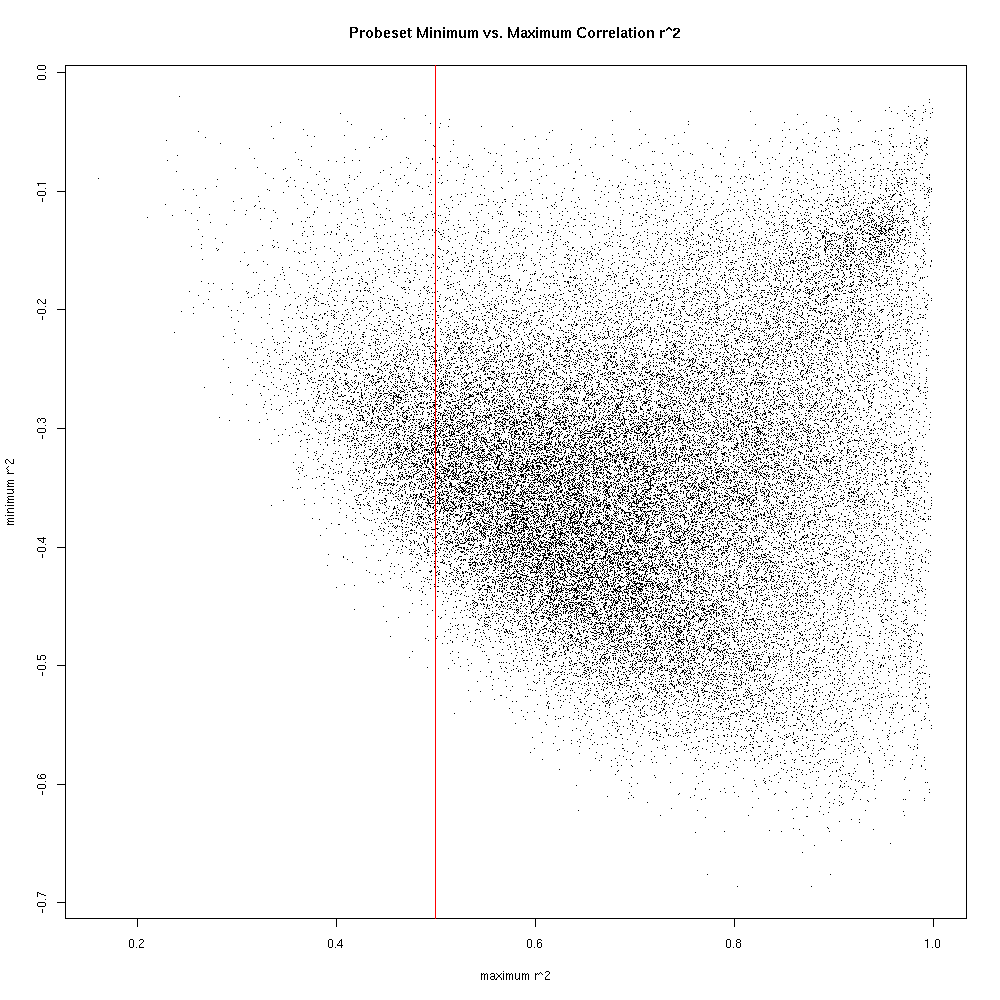
\includegraphics[width=12cm]{mincor_maxcor.png}
\caption{Correlation $r^2$ Minima vs. Maxima, All Probesets.}
\end{figure}
%\pagebreak

%XXX
\begin{figure}[htbp]
\label{figure:bp_annot}
%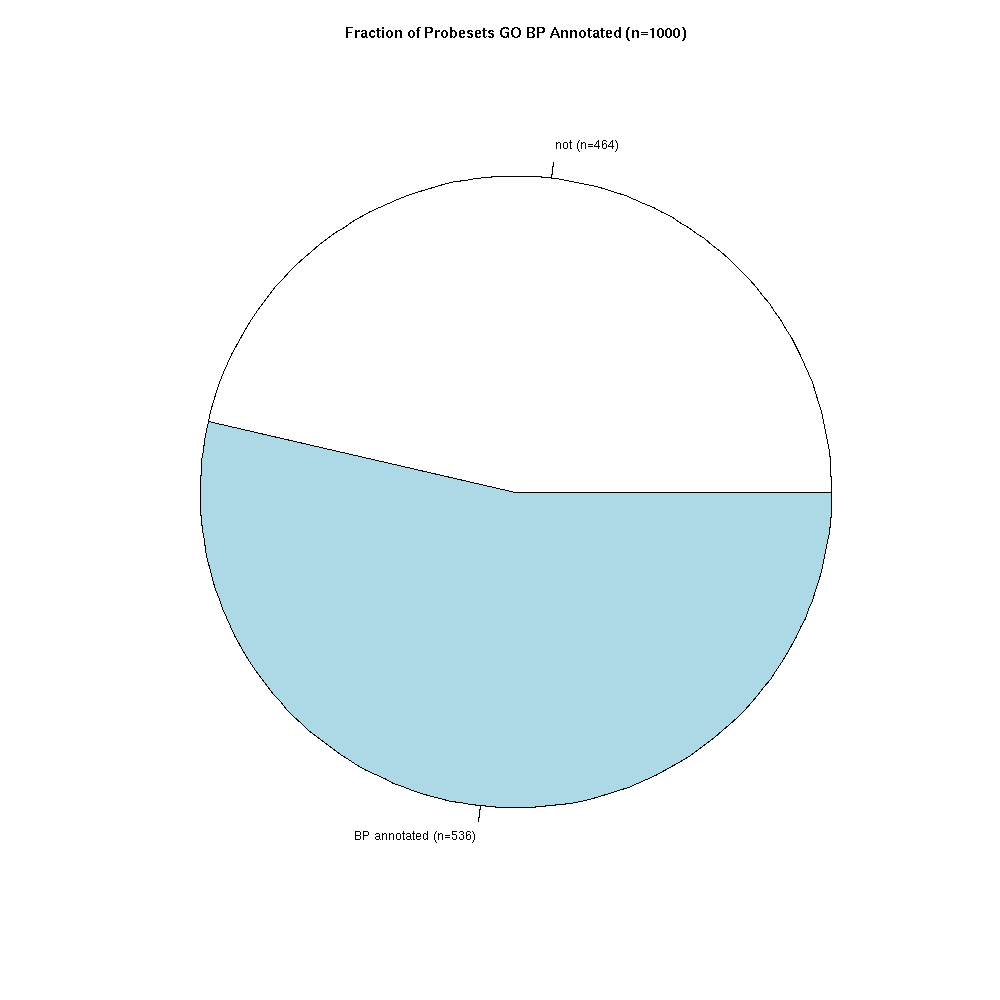
\includegraphics[width=12cm]{bp_annot.png}
\caption{Fraction of Annotated Probesets.}
\end{figure}
%\pagebreak

%XXX
\begin{figure}[htbp]
\label{figure:bp_recall}
%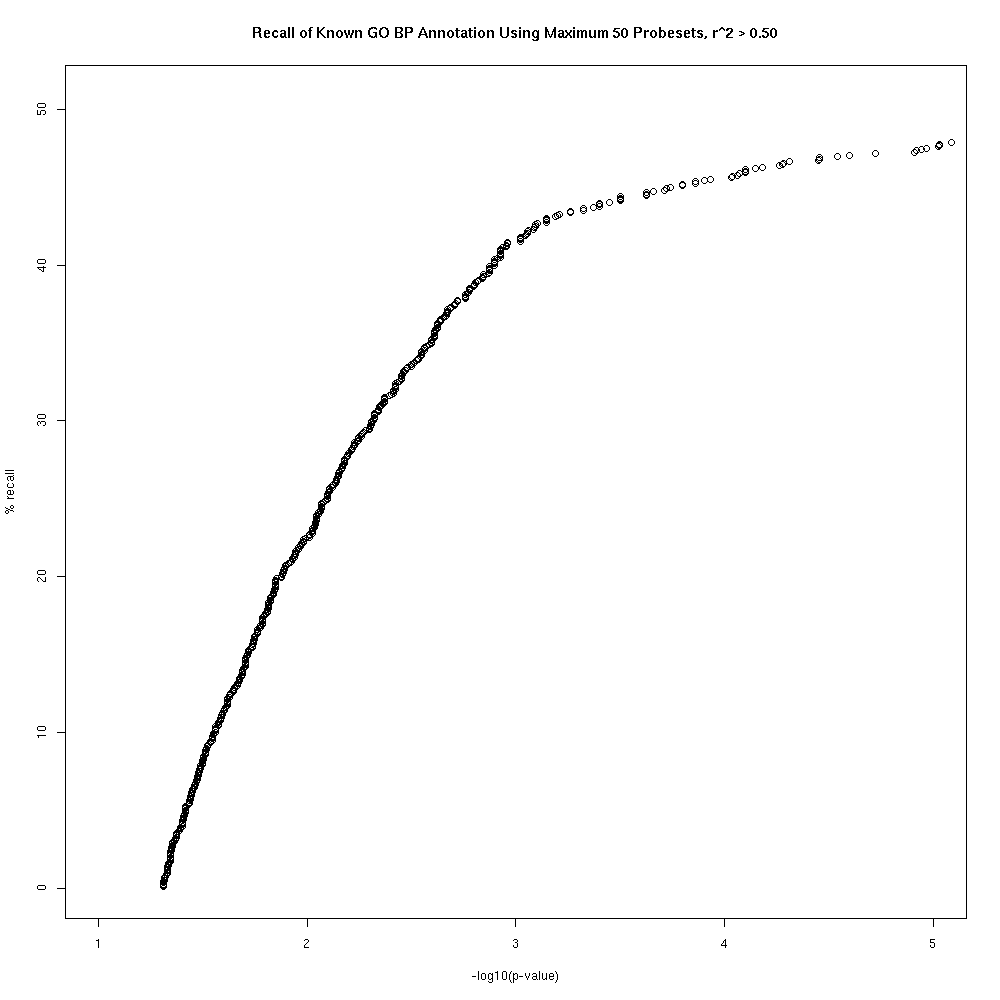
\includegraphics[width=12cm]{bp_recall.png}
\caption{Recall of Known Annotation.}
\end{figure}
%\pagebreak

%XXX
\begin{figure}[htbp]
\label{figure:bp_novel}
%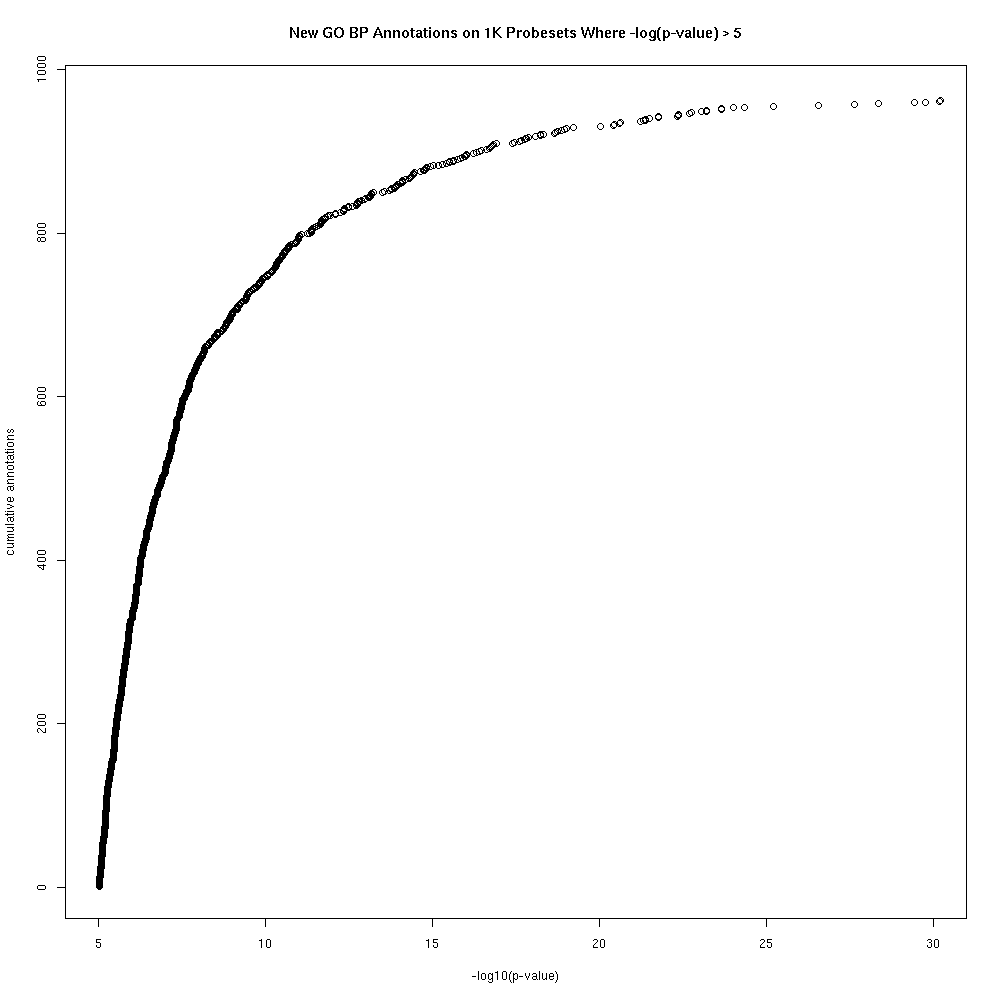
\includegraphics[width=12cm]{bp_novel.png}
\caption{P-values of High-Quality, Novel Annotation.}
\end{figure}
%\pagebreak

\end{document}
